\documentclass[16pt,spanish]{article}
\usepackage[utf8]{inputenc}
\usepackage{graphicx}
\usepackage{mathtools}

\author{
	Joaquín Cerviño\\
	\and
	Tutor: Esteban Calcagno\\
}

\title{Seminario de investigación: }
\subtitle{Técnicas generativas para la producción audiovisual en entornos digitales}

\begin{document}

\maketitle
\pagenumbering{gobble}
\newpage
\pagenumbering{arabic}

\section{Autómata Celular}
\subsection{Introducción}

		Los autómatas celulares(AC) fueron concebidos por Stanislaw Ulam y John von
Neumann a partir de análisis realizados sobre desarrollos morfológicos.(falta cita) Los AC son
sistemas complejos que pueden manifestar un comportamiento global o emergente.
Coveney y Highfield definen a una propiedad emergente como “una propiedad de un
sistema complejo que consiste de varias unidades que interactúan” (Coveney,Highfield,
1995)~\cite{highfield1996frontiers}. Estos sistemas fueron objeto de estudio durante años, contando entre sus
estudiosos a científicos como Konrad Zuse(1969), Ed Fredkin(1992) y Stephen
Wolfram(1984)(faltan citas). Cabe destacar que este último hizo uno de los desarrollos y análisis más
extensos sobre el tema. 		

		Wolfram define a los autómatas celulares como ``una línea de celulas, cada una coloreada de negro o blanco, representando dos estados posibles. El estado de cada célula se evalúa a cada paso, puediendo permanecer en su estado previo o cambiar su condición, de acuerdo a una regla definida que toma por parámetros la condición de las dos células vecinas en el paso anterior"(Wolfram,2002)~\cite{wolfram2002new}. El autor destaca que los autómatas celulares son capaces de manifestar un comportamiento altamente complejo pese a que se comporten según una regla simple y hayan partido de un estado inicial igualmente simple. (Mostrar imagenes) 
		
		
\begin{figure}[h!]
\begin{subfigure}[a]{0.5\linewidth}
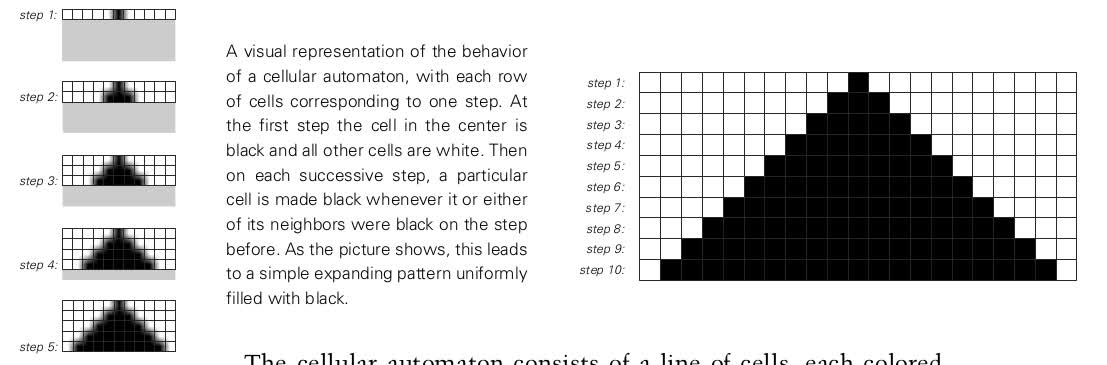
\includegraphics[width=\linewidth]{imagesCA/Example-1-a.jpg}
\caption{Algo.}
\end{subfigure}
\begin{subfigure}[b]{0.5\linewidth}
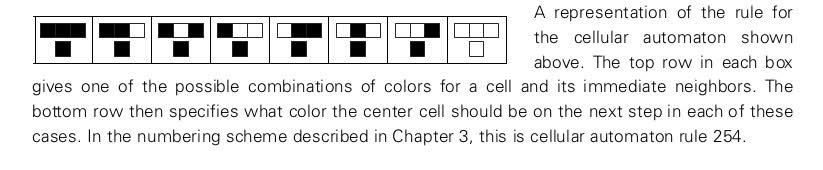
\includegraphics[width=\linewidth]{imagesCA/Example-1-b.jpg}
\caption{Algo.}
\end{subfigure}
\end{figure}

\begin{figure}[h!]
\begin{subfigure}[c]{0.5\linewidth}
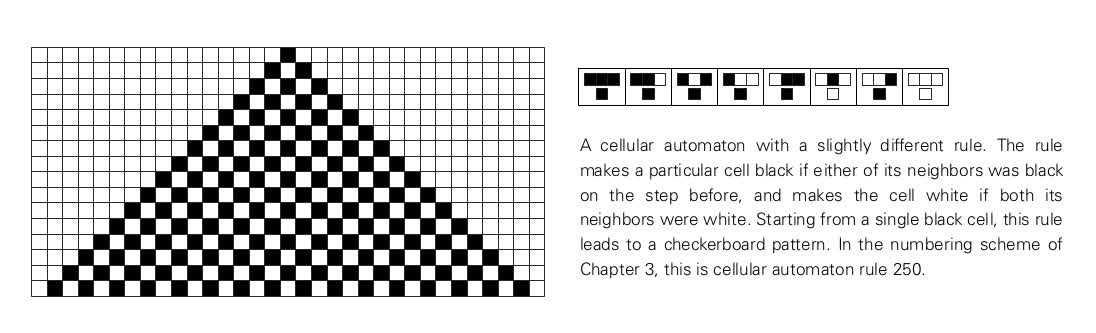
\includegraphics[width=\linewidth]{imagesCA/Example-2.jpg}
\caption{Algo.}
\end{subfigure}
\begin{subfigure}[d]{0.5\linewidth}
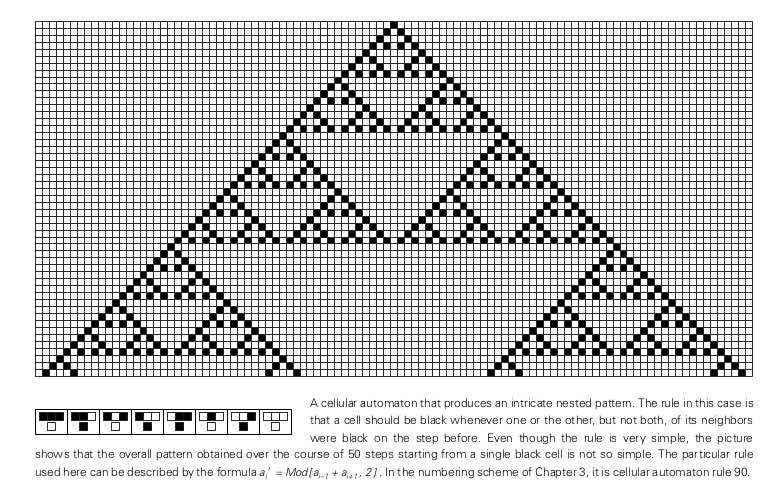
\includegraphics[width=0.5\linewidth]{imagesCA/Example-3.jpg}
\caption{Algo.}
\end{subfigure}
\end{figure}

	A partir de la observación realizada sobre los resultados de distintas tipos de autómatas celulares, es decir, basados en distintas reglas, y provenientes de estados iniciales aleatorios, Wolfram llega a la conclusión que el comportamiento emergente de éstos puede ser clasificados en cuatro grupos. Éstos a su vez están ordenados según un grado creciente de complejidad.


\begin{figure}[h!]
	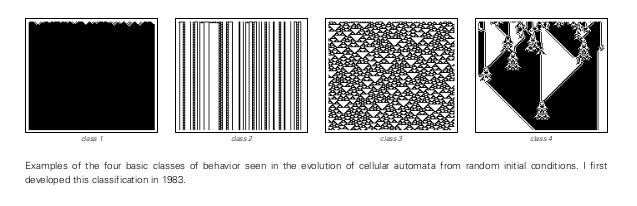
\includegraphics[width=\linewidth]{imagesCA/clasificacion.jpg}
\endfigure


	El primer grupo es el que exhibe el comportamiento más simple y en éste se incluyen a los AC que desde cualquier punto inicial derivan en un mismo estado final uniforme. 
	En el segundo grupo, hay varios estados finales pero todos éstos permanecen inalterados o se repiten luego de un número reducido de pasos. 
	En el tercer grupo el comportamiento es más complejo y es en su gran mayoría aleatorio, aunque puedan ocurrir pequeñas estructuras como triángulos de forma esporádica.
	En el cuarto grupo, se agrupan a los AC que muestran un comportamiento que resulta de una mezcla de aleatoriedad y orden. En esta categoría se pueden observar la aparición de pequeñas estructuras que a su vez interactúan con otras de un forma compleja.		

\subsection{Estudios de caso}
	
\subsubsection{Chaossynth}
	La síntesis granular es una técnica que fue conceptualizada por primera vez por Xenakis en su libro Musiques Formelles(1981)~\cite{xenakis1981musiques}. Las primeras implementaciónes se puedieron hacer con el advenimiento de la síntesis digital, siendo Curtis Roads(1991)~\cite{roads1991asynchronous} y Truax(1988)~\cite{truax1988real} los primeros en experimentar e implementar esta técnica. Posteriormente, Roads le otorgó un marco conceptual y académico que quedó plasmado en su libro Microsound(2004)~\cite{roads2004microsound}. Esta técnica consiste en la utilización de un gran número ``granos" (sonidos de muy corta duración, por ejemplo, de hasta 50 milisegundos), que pueden tener variadas formas de onda y a los cuales se les aplica una envolvente. La masa generada como resultado de la sumatoria de granos tiene parámetros globales que la determinan, como por ejemplo, la densidad. En este aspecto Xenakis propone modelos estocásticos para modelar la morfología de estas nubes de granos. Eduardo Reck Miranda(1995)~\cite{miranda1995granular} propone la utilización de autómatas celulares para controlar la producción de granos en la síntesis granular a través del Chaossynth.
	ChaOs proviene de la expresión \textit{Chemical Oscillator}, ``una representación metafórica de un fenómeno neurofisiológico conocido como circuito de reverberación neuronal"(Miranda, 1995). En este caso, las células que componen al AC son interpretadas como células nerviosas que pueden manifestar tres estados: inactivo(\textit{quiescent}), despolarizado(\textit{depolarized}) o quemado(\textit{burned state}). Este AC evoluciona de un estado incial de completa aleatoriedad a un comportamiento oscilatorio donde pueden discernirse patrones. Miranda plantea que esta característica emergente del sistema es similar a cómo se producen sonidos de forma natural en instrumentos acúsitcos ya que, al igual que el AC, ``los sonidos tienden a converger de una amplia distribución de sus parciales(por ejemplo ruido) a patrones ocilatorios(por ejemplo, un sonido armónico)". En el Chaossynth la interacción entre células representa la circulación de corriente entre ellas. Hay dos umbrales con distintos valores, uno con un valor de voltaje mínimo(Vmin) y otro con un valor máximo(Vmax). Si el valor del voltaje de la célula se encuentra por debajo del Vmin, la célula se encuentra en estado inactivo(o ``polarizada"); si su valor está entre Vmin inclusive y Vmax está despolarizada. Cada célula ``tiene un divisor de potencia(\textit{potiential divider}) cuya finalidad es mantener el voltaje de la misma debajo de Vmin. Si el divisor falla, esto es, si Vi alcanza Vmin, la célula nerviosa se despolariza. También, está en juego un capacitor eléctrico que regula la velocidad de despolarización." Miranda destaca que la tendencia global del sistema es a que la células se despolaricen cada vez más con el transcurrir del tiempo, o a cada paso. Por último, se aclara que ``una célula quemada en el tiempo(o paso t) es reemplazada por una nueva célula inactiva en el siguiente paso(t+1)".

A modo de resumen, se puede inferir que el comportamiento del ChaOs depende de los siguientes factores:

1) El número n de estados, siendo n > 3.

2) El valor de las resistencias r1 y r2 del divisor de potencia.

3) La capacitancia k del grado de depolarización.

4) La velocidad t del sistema.

5) La dimensión de la grilla.


El Chaosynth hace uso del comportamiento del sistema anteriormente descripto(ChaOs) para manejar la generación de un gran número de ``partículas sonoras" para formar un evento sonoro complejo. Miranda hace uso de lo que el llama \textit{Mapping Technique}(técnica de mapeo) para utilizar el ChaOs con el fin de secuenciar partículas sonoras, o ``granos". Cada una de estas partículas  ``está compuesta por varios parciales. Cada parcial es una sinusoide generada por un oscilador. Un oscilador necesita tres parámetros para funcionar: frecuencia, amplitud y duración(en milisegundos). ChaOs controla los valores de frecuencia y la duración de la partícula, pero los valores de amplitud son establecidos por el usuario de forma previa. Los estados de una célula nerviosa están asociados a un valor de frecuencia y los osciladores están asociados a un cierto número de células. Los valores de frecuencia en un tiempo t son, por consiguiente, establecidos por el promedio de las frecuencias asociados a los estados de la célula nerviosa mapeada a cada oscilador"(Miranda,1995). En el Chaosynth se permite al usuario establecer otros parámetros como por ejemplo, el tamaño de la grilla, la cantidad de osciladores, la relación entre células nerviosas y osciladores y lo parámetro internos del ChaOS(el número de estados, el valor de las resistencias, la capacitancia de las células). En cuanto a la síntesis de sonido se puede agregar que es en escencia aditiva, ya que cada partícula sonora o ``grano" es generados por la unión de varias sinusoides.


\begin{figure}[h!]
\begin{subfigure}[f]{0.5\linewidth}
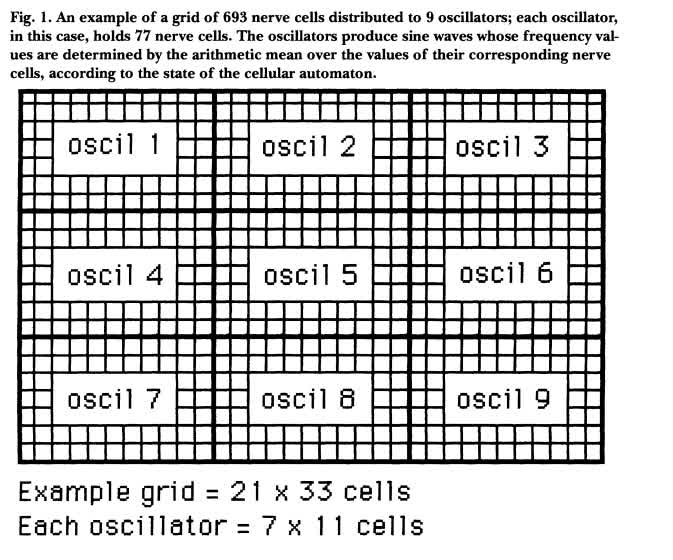
\includegraphics[width=0.5\linewidth]{imagesCA/mapping_technique.jpg}
\caption{Técnica de mapeo.}
\end{subfigure}
\begin{subfigure}[g]{0.5\linewidth}
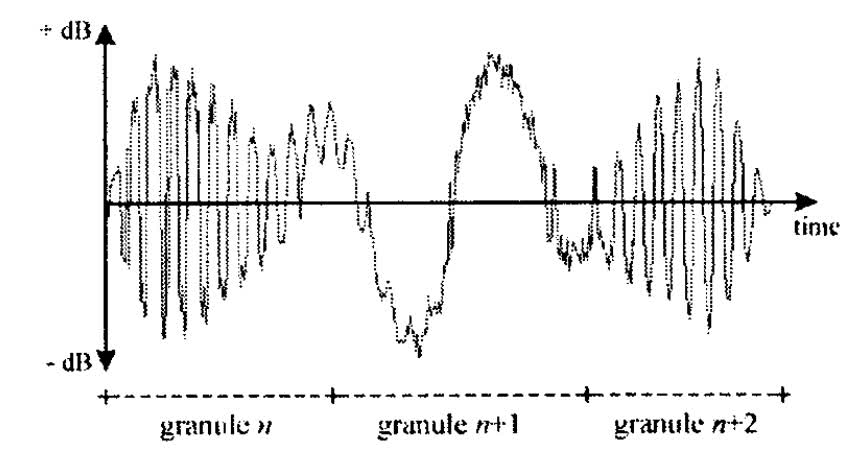
\includegraphics[width=0.5\linewidth]{imagesCA/Granular_output.jpg}
\caption{Resultado obtenido por el Chaosynth.}
\end{subfigure}
\end{figure}


\subsubsection{Implementación}

	El Chaosyth se trata de un autómata celular de dos dimensiones. La representación varía en comparación a los expuestos en la introducción en que lo que se grafica es un estado actual en una grilla de células, en contraposición al de una serie de pasos consecutivos. La implementación del Chaosynth en Processing está basada en la de Daniel Shiffman del \textit{Game of Life} de John Conway. El juego desarrollado por dicho matemático consiste en un tablero con casilleros que pueden estar ocupados o no por fichas, que representan organismos ``vivos", que se trasladan de acuerdo a ``leyes genéticas". Esta clase de juegos se denominan de  ``simulación"(\textit{Simulation game}) ya que exhiben un desarrollo análogo a aquellos de seres vivos. Las reglas estipuladas por el creador del juego fueron hechas para que satisfagan las siguientes tres normas: ``1. No debe haber un patrón inicial[de células] mediante el cual pueda haber una propagación sin límite de células. 2. Debe haber parámetros iniciales que aparentemente crezcan sin límite. 3. Debe haber un patrón inicial simple que crezca y se transforme durante un tiempo considerable y llegue a tres finales posibles: desaparecer completamente (por superpoblación o escasez), permanecer en una configuración estable que permanece sin cambios, o entrar en una fase oscilatoria en la cual se repitan patrones de forma permanente cada dos o tres ciclos".~\cite{gardner1971mathematical} Shiffman interpreta que el \textit{Game of Life} se trata de un autómata celular de clase 4 según la taxonomía de Wolfram.~\cite{shiffman2012nature}. Como el Chaosynth representa metafóricamente a un oscilador químico en el cual células se despolarizan o queman, el Game of Life representa el desarrollo de organismos que nacen, mueren o sobreviven según el estado de las células vecinas: ``1. Supervivencia. Cada ficha [célula] que contenga dos o tres células adyacentes sobrevive a la siguiente generación. 2. Muertes. Cada célula que posea cuatro o más vecinos muere por superpoblación. Cada, célula con un solo vecino o ninguno muere por su aislamiento. 3. Nacimientos. Cada célula muerta o casillero vacío con exactamente tres células adyacentes vivas nace, esto es, ese casillero posee una célula viva en la siguiente generación".~\cite{gardner1971mathematical} El Chaosynth es una extensión del Game of Life con otras reglas y con más estados posibles para las células.


\begin{figure}[h!]
\begin{subfigure}[h]{0.5\linewidth}
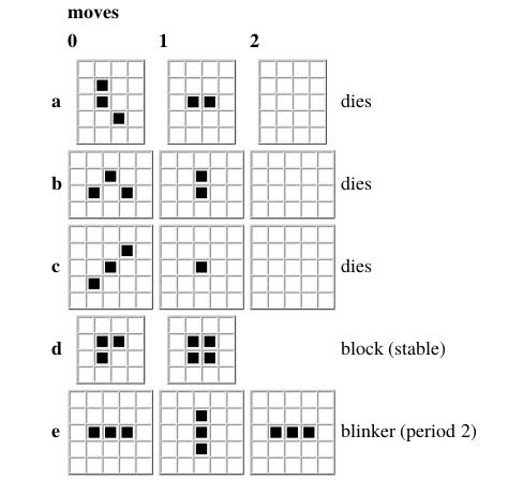
\includegraphics[width=0.5\linewidth, bb= 0 0 640 480]{imagesCA/gol_1a.jpg}
	\caption{Ejemplo del funcionamiento del \textit{Game of Life}.}
\end{subfigure}
\begin{subfigure}[i]{0.5\linewidth}
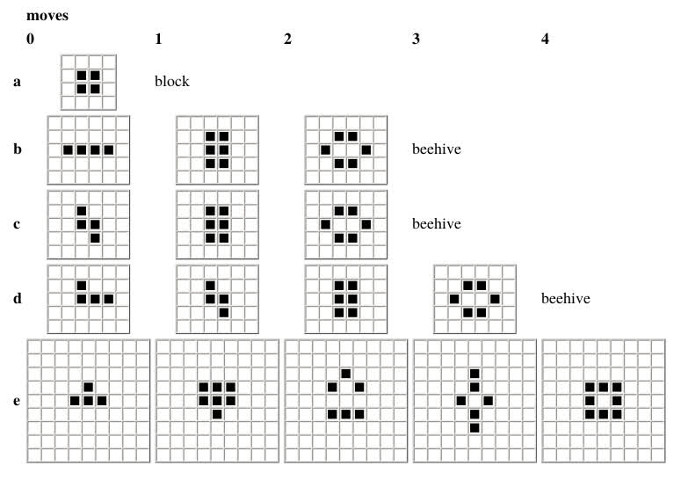
\includegraphics[width=0.5\linewidth, bb = 0 0 640 480]{imagesCA/gol_2a.jpg}
\caption{Patrones que emergen del \textit{Game of Life}, como el ``panal de abejas".}
\end{subfigure}
\end{figure}

	 
Seguir con granular sinthesis celular automaton

\newpage
\bibliography{sketch.bib}
\bibliographystyle{plain}

\end{document}
